\documentclass[floatsintext,man]{apa6}

\usepackage{amssymb,amsmath}
\usepackage{ifxetex,ifluatex}
\usepackage{fixltx2e} % provides \textsubscript
\ifnum 0\ifxetex 1\fi\ifluatex 1\fi=0 % if pdftex
  \usepackage[T1]{fontenc}
  \usepackage[utf8]{inputenc}
\else % if luatex or xelatex
  \ifxetex
    \usepackage{mathspec}
    \usepackage{xltxtra,xunicode}
  \else
    \usepackage{fontspec}
  \fi
  \defaultfontfeatures{Mapping=tex-text,Scale=MatchLowercase}
  \newcommand{\euro}{€}
\fi
% use upquote if available, for straight quotes in verbatim environments
\IfFileExists{upquote.sty}{\usepackage{upquote}}{}
% use microtype if available
\IfFileExists{microtype.sty}{\usepackage{microtype}}{}

% Table formatting
\usepackage{longtable, booktabs}
\usepackage{lscape}
% \usepackage[counterclockwise]{rotating}   % Landscape page setup for large tables
\usepackage{multirow}		% Table styling
\usepackage{tabularx}		% Control Column width
\usepackage[flushleft]{threeparttable}	% Allows for three part tables with a specified notes section
\usepackage{threeparttablex}            % Lets threeparttable work with longtable

% Create new environments so endfloat can handle them
% \newenvironment{ltable}
%   {\begin{landscape}\begin{center}\begin{threeparttable}}
%   {\end{threeparttable}\end{center}\end{landscape}}

\newenvironment{lltable}
  {\begin{landscape}\begin{center}\begin{ThreePartTable}}
  {\end{ThreePartTable}\end{center}\end{landscape}}




% The following enables adjusting longtable caption width to table width
% Solution found at http://golatex.de/longtable-mit-caption-so-breit-wie-die-tabelle-t15767.html
\makeatletter
\newcommand\LastLTentrywidth{1em}
\newlength\longtablewidth
\setlength{\longtablewidth}{1in}
\newcommand\getlongtablewidth{%
 \begingroup
  \ifcsname LT@\roman{LT@tables}\endcsname
  \global\longtablewidth=0pt
  \renewcommand\LT@entry[2]{\global\advance\longtablewidth by ##2\relax\gdef\LastLTentrywidth{##2}}%
  \@nameuse{LT@\roman{LT@tables}}%
  \fi
\endgroup}


  \usepackage{graphicx}
  \makeatletter
  \def\maxwidth{\ifdim\Gin@nat@width>\linewidth\linewidth\else\Gin@nat@width\fi}
  \def\maxheight{\ifdim\Gin@nat@height>\textheight\textheight\else\Gin@nat@height\fi}
  \makeatother
  % Scale images if necessary, so that they will not overflow the page
  % margins by default, and it is still possible to overwrite the defaults
  % using explicit options in \includegraphics[width, height, ...]{}
  \setkeys{Gin}{width=\maxwidth,height=\maxheight,keepaspectratio}
\ifxetex
  \usepackage[setpagesize=false, % page size defined by xetex
              unicode=false, % unicode breaks when used with xetex
              xetex]{hyperref}
\else
  \usepackage[unicode=true]{hyperref}
\fi
\hypersetup{breaklinks=true,
            pdfauthor={},
            pdftitle={The Acoustics of Shouting: A Case Study of English Vowels},
            colorlinks=true,
            citecolor=blue,
            urlcolor=blue,
            linkcolor=black,
            pdfborder={0 0 0}}
\urlstyle{same}  % don't use monospace font for urls

\setlength{\parindent}{0pt}
%\setlength{\parskip}{0pt plus 0pt minus 0pt}

\setlength{\emergencystretch}{3em}  % prevent overfull lines


% Manuscript styling
\captionsetup{font=singlespacing,justification=justified}
\usepackage{csquotes}
\usepackage{upgreek}

 % Line numbering
  \usepackage{lineno}
  \linenumbers


\usepackage{tikz} % Variable definition to generate author note

% fix for \tightlist problem in pandoc 1.14
\providecommand{\tightlist}{%
  \setlength{\itemsep}{0pt}\setlength{\parskip}{0pt}}

% Essential manuscript parts
  \title{The Acoustics of Shouting: A Case Study of English Vowels}

  \shorttitle{The Acoustics of Shouting}


  \author{Dine Mamadou}

  % \def\affdep{{""}}%
  % \def\affcity{{""}}%

  \affiliation{
    \vspace{0.5cm}
          \textsuperscript{} Rutgers University  }



  



  \usepackage{tipa}
  \usepackage{gb4e}
  \noautomath
  \usepackage{natbib}
  \usepackage{apalike}

\usepackage{amsthm}
\newtheorem{theorem}{Theorem}[section]
\newtheorem{lemma}{Lemma}[section]
\theoremstyle{definition}
\newtheorem{definition}{Definition}[section]
\newtheorem{corollary}{Corollary}[section]
\newtheorem{proposition}{Proposition}[section]
\theoremstyle{definition}
\newtheorem{example}{Example}[section]
\theoremstyle{definition}
\newtheorem{exercise}{Exercise}[section]
\theoremstyle{remark}
\newtheorem*{remark}{Remark}
\newtheorem*{solution}{Solution}
\begin{document}

\maketitle

\setcounter{secnumdepth}{0}



\subsection{Introduction}\label{introduction}

The current paper is an investigation of the acoustic properties of
English vowels in shouted utterances; that is, we investigated whether
or not vowel quality is affected in those utterances. Shouting is very
demanding on the vocal tract and as such may cause the latter to undergo
distortions of its shape. In this regards, the Source and Filter theory
makes interesting predictions on the potential effects of yelling on
vowel quality. Acording to this theory, speech sounds are distinguished
on the basis of both the source and filter properties of the vocal tract
(Maddieson 1984, Diehl 2008). That is, different configurations of the
vocal tract and the activity of the glottis as the source will yield
different vowel qualities.

So, if yelling has a distorting effect on the shape of the vocal tract,
then the resulting sound will reflect the changes in the shape of the
filter meaning the vowels under observation would display qualities that
differ from vowel sounds that are normally uttered. In fact, Huber \& al
(1999) found that higher vocal intensities (a correlate of loudness) are
typically produced with an increased jaw opening with a co-occurring
decreased tongue height which in turn results in an increased F1. This
predicts that vowels in shouting will be higher than those in normally
uttered speech. Additionally, we can further predict that the
transitions of the articulators in the course of a shouted utterance may
take more time than they do in normal utterance; yielding longer vowels
in the former condition than in the latter.

Ladefoged \& Johnson (2011:92), point out that in English, \enquote{the
first part of the diphthong is usually more prominent than the last.
(\ldots{}) the diphthongs often do not begin and end with any of the
sounds that occur in simple vowels.} Assume that the prominence of the
first part of the diphthong is due to its position in the articulation
chain, the higher the energy involved in an articulation process, the
more peripheral the sound is likely to be. If this correlation is
verified, the vowels involved in shouted diphthongs will have formant
values that are closer to those of the monophthong versions of those
vowels.

Building on the predictions of the discussion above, we hypothesize
that:

H1: Vowel F1 will crease as a functon of intensity and

H2: Duration will be a good predictor of shouting.

\subsection{Participants}\label{participants}

Two native speakers of English (1 Male and 1 Female) from Iowa and
Illinois, respectively were recorded. The female participant is a
monolingual while the male participant speaks German (at an intermediate
level) in addition to English. Both were informed of the comaprative
purpose of the study but knew very little to nothing about the different
points of comparison. The participants were recorded in a soundproof
booth using \textbf{PMD661MKII Handheld Solid State Recorder}. The
detachable microphone of the recorder was mounted to the participants'
heads to ensure the distance between their mouth and the microphone is
kept consistent at all time during the recording sessions. The
recordings were done in mono and outputed in .wav format. In the shouted
condition, the loudness threshold was set twice as high as the loudness
threshold of the normal condition to prevent the higher frequences from
being cut off.

\subsection{Experimental design}\label{experimental-design}

The participants produced 16 randomized target words, comprised of 10
monophthongs and 6 diphthong in \textbf{hVd} context (an adaptation from
Yoon \& al., 2012). The 16 target words contain the monophthongs
\textbf{{[}\textipa{i, I, E, A, O, u, \textrhookschwa, \textturnv, \ae, U}{]}},
and the diphthongs \textbf{{[}\textipa{eI, OI, oU, ju, aI, aU}{]}}. Shwa
was not included because it we could not find a word with schwa in the
hVd context.

The items were produced in two conditions: \enquote{normal} and
\enquote{shouted}. In the former condition, they were instructed to
speak the way they would normally speak in a conversation with a person
right in front of them, while in the latter, the instruction was to
speak as though they were talking to a person who is about 100m away
from them.

Each token was repeted twice in each condition, yielding a total of
\textbf{128 target tokens}. The target words were pronounced in
isolation, as opposed to in a frame sentence, in order to minimize
tiredome of participants, especially in the shouted condition.

\subsection{Measurements and Material}\label{measurements-and-material}

F1, F2, Intensity and vowel duration measurements were harvested in
Praat (version 6.0.32) using a script by Mietta Lennes (version
4.7.2003). F1, F2 and intensity measurements were taken at the midpoint
of the middle 1/3 (at the steady state) of the vowels. Vowel duration
was measured from the first zero crossing of the first harmonic of the
vowel to the last zero crossing of the last harmonic before the stop
closure (determined simultaneously on the basis of the waveform and the
spectogram). Because each target word had a voiced coda, which have a
robust second formant, the onset of the coda consonant closure was used
as the right interval since it is more reliable than the offset of F2 in
this case. Only the monophthongs are reported here.

The praat TextGrid was annotated in three tiers, the Formant tier, the
Intensity tier and the duration tier. Each interval on each tier was
encoded for the Condition (Normal and shouted) Vowel, Gender (Male and
Female), Repetition (First = 1, Second = 2).

\subsection{Data Analysis}\label{data-analysis}

The collected data was analysed in R (Version 3.4.3; R Core Team, 2017).
Two sets of nested generalized linear models were fitted using the R
function \textbf{glm()} with the Gaussian distribution family and
\enquote{identity} as the link; under the assumption that the data is
normally distributed. This assumption was later confirmed by eyeballing
the normality and homoskedasticity of the plots of the variables. In
order for our models to reflect our hypotheses, F1 was set as the
criterion in one set of nested models and Duration in the other.

The predictors were both continuous (Intensity, (F1) and
(duration))\footnote{When F1 is the criterion, it's removed from the predictors; same for duration.}
and categorical (gender). Models with the same criterion were compared
via the \textbf{anova()} function. In models with main effects and
interaction, R\^{}2 was obtained using the function
\textbf{r.squaredGLMM()}. Experiment-wise alpha was set at
\textbf{0.05}.

\subsection{Results and Discussion}\label{results-and-discussion}

A descriptive summary of the data is presented in \emph{Table1} below.
F1 is in average \emph{140Hz (214.89HZ)} higher in the shouted condition
than it is in the normal condition, while intensity showed to be
\emph{5Hz} more in the former than in the latter. As far as duration is
concerned, vowels are almost twice as long (\emph{27ms vs 43ms}) when
shouted than when normally spoken.

\begin{tabular}{l|r|r|r|r|r|r}
\hline
condition & meanf1 & sd.f1 & mean.int & sd.int & mean.dur & sd.dur\\
\hline
Normal & 598.47 & 214.89 & 75.46 & 2.56 & 0.27 & 0.08\\
\hline
Shouted & 740.90 & 198.32 & 80.06 & 4.53 & 0.43 & 0.15\\
\hline
\end{tabular}

\emph{Table1: This table shows the descriptive statistics of the data.}

In the nested model with F1 as the criterion, a main effect of Gender
was found (p\textless{}0.05) with an \emph{R\^{}2} of \emph{0.18}
(R\^{}2 of centered measurements). Intensity was almost significant
(p=0.08). More importantly, however, an interaction between gender and
intensity was found (p\textless{}0.05) and the variance explained is
\emph{R\^{}2=0.28}. That is, F1 increases as funtion of intensity based
on gender.

In the nested model with duration as the criterion, gender was also
found to have a main effect (p\textless{}0.05) with a variance explained
of \emph{0.18} (again in centered values). An interaction was also
observed between intensity and gender (p\textless{}0.05) with an R\^{}2
of \emph{0.54}. The two nested models indicate that intensity is a good
predictor of F1 and duration only if modulated by gender. More
precisely, intensity is a good predictor of F1 in males while it only
correlates with duration with females.

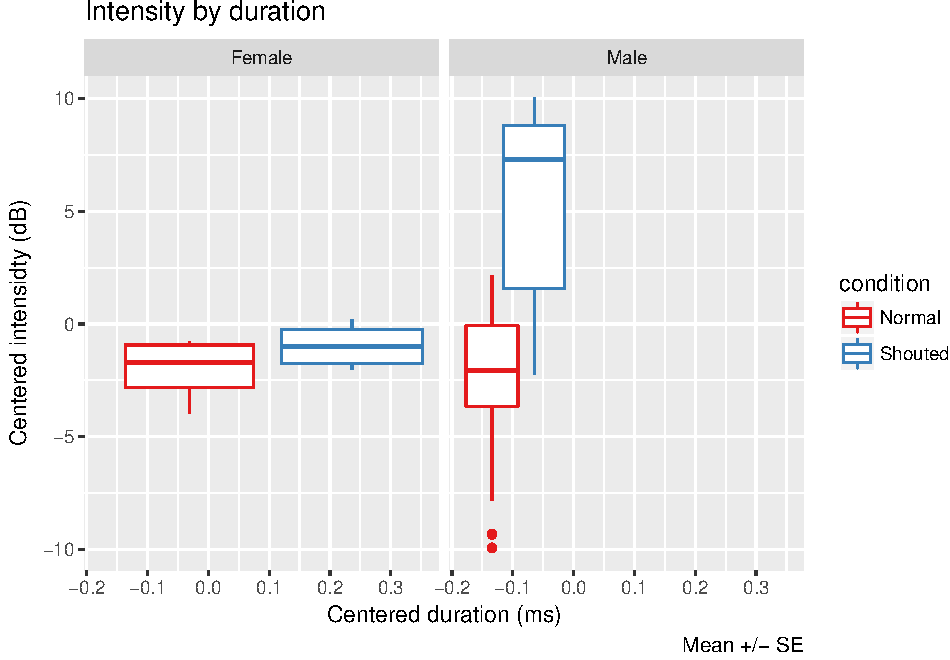
\includegraphics{shouted_files/figure-latex/Figure1-1.pdf}
\emph{Figure1: This figure shows Intensity as a function of Duration by
gender. In the shouted condition, Female vowel length is about
0.25(centered ms) while male's is only -0.12. Male compensate this by
having a higher intensity value (7.5 in centered ms) while female's is
slightly under o.}

In both sets of models, the models with interaction offered the best fit
for the data. While this did not exactly validate neither of our
hypothesis, it did show that intensity alone is not a good predictor of
vowel height (F1). This finding also partially aligns with Huber \& al.
(1999) in that only the Male speaker have higher vowels as a function of
an increase in intensity, on one hand. On the other, the Female speaker
does not use intensity as a cue for loudness, she uses vowel duration
instead (\emph{See Figure2 below}).

\newpage

\begin{figure}
\centering
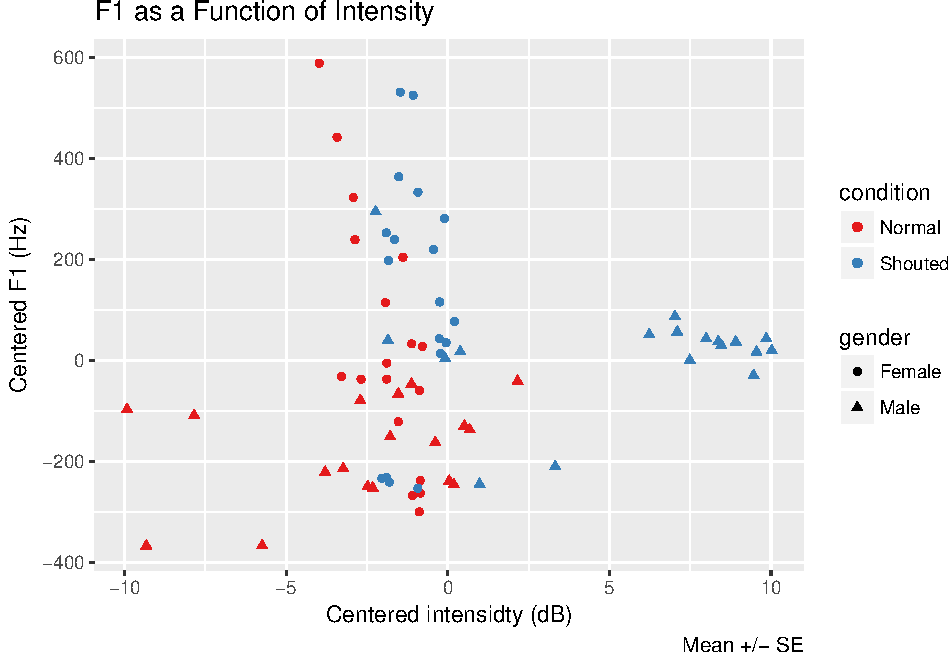
\includegraphics{shouted_files/figure-latex/Figure4-1.pdf}
\caption{}
\end{figure}

\subsection{Conclusion}\label{conclusion}

This paper investigated whether or not there's a difference in vowel
quality between shouted and normally spoken speech in Female and Male.
The findings supported the intution that there is indeed a difference.
However, unlike a direct correlation between vowel heigh (F1) and
intensity as suggested in the literature (namely Huber \& al. (1999)),
we found a more nuanced correlation. That is, Male speakers use
intensity as a systematic cue for loudness and showed an increase in F1
as intensity increased. The Female speaker on the other hand
systematically used vowel duration as a cue for loudness and only
secondarily used intensity. While this systematic difference may reflect
sociological and gender approaches to loudness, it highlights the
importance of a gender sensitivity approach to these kinds of studies
and constitutes a base on which future work can build.

\newpage

\subsection{References}\label{references}






\end{document}
